\documentclass[manuscript=article]{achemso}

\usepackage{amsmath}
\usepackage{booktabs}
\usepackage{graphicx}
\usepackage{microtype}
\usepackage{xcolor}
\usepackage{array}
\usepackage{caption}
\usepackage{placeins}
\usepackage{xurl}

\captionsetup{font=small,labelfont=bf}
\setlength{\tabcolsep}{6pt}
\renewcommand{\arraystretch}{1.12}


\newcommand{\DataSummaryTable}{%
\begin{table}[!htbp]
\centering
\caption{Prepared ChEMBL 36 activity dataset and fold-0 split.}
\label{tab:data-summary}
\begin{tabular}{lr}
\toprule
Quantity & Value \\
\midrule
Raw activity rows queried & 3,501,718 \\
Canonical molecules after filtering and deduplication & 1,369,515 \\
Binary activity threshold & pChEMBL $\geq$ 7.0 \\
Active molecules & 520,188 \\
Temporal holdout molecules & 274,541 \\
Fold-0 training molecules & 875,979 \\
Fold-0 internal-validation molecules & 218,995 \\
\bottomrule
\end{tabular}
\end{table}
}

\newcommand{\ModelPerformanceTable}{%
\begin{table}[!htbp]
\centering
\caption{Activity-model performance on ChEMBL 36 holdouts.}
\label{tab:model-performance}
\begin{tabular}{lrrrr}
\toprule
Split & RMSE & $R^2$ & Spearman & EF@1\% \\
\midrule
Internal validation & 0.8466 & 0.5992 & 0.7674 & 2.7331 \\
Temporal holdout & 1.1615 & 0.2473 & 0.5171 & 2.4359 \\
\bottomrule
\end{tabular}
\end{table}
}

\newcommand{\BaselineSanityTable}{%
\begin{table}[!htbp]
\centering
\caption{Selected baseline sanity checks, not a full benchmark suite. Random forest and Chemprop use sampled ChEMBL 36 splits for context only; they are not full-dataset, same-protocol baselines. The current model and previous so\_f4 comparison use the full future prediction artifacts.}
\label{tab:baselines}
\begin{tabular}{llrrrr}
\toprule
Model & Evaluation rows & RMSE & $R^2$ & Spearman & EF@1\% \\
\midrule
Current 2D MLP & Future full (274,541) & 1.1615 & 0.2473 & 0.5171 & 2.4359 \\
Previous so\_f4 & Future full (274,541) & 1.1914 & 0.2080 & 0.4806 & 2.1008 \\
Random forest Morgan & Future sample (10,000) & 1.2236 & 0.1736 & 0.4203 & 1.9859 \\
Chemprop D-MPNN & Future sample (10,000) & 1.2164 & 0.1834 & 0.4337 & 1.8100 \\
\bottomrule
\end{tabular}
\end{table}
}

\newcommand{\BaceOverlapTable}{%
\begin{table}[!htbp]
\centering
\caption{BACE external-source performance before and after fold-0 training-overlap control. Primary interpretation should use the strict scaffold-disjoint row.}
\label{tab:bace-overlap}
\begin{tabular}{lrrrrr}
\toprule
Subset & $n$ & ROC AUC & RMSE & Spearman & EF@1\% \\
\midrule
Full, provenance only & 1513 & 0.8304 & 0.9330 & 0.6958 & 2.0527 \\
Structure-disjoint & 1192 & 0.8035 & 1.0052 & 0.6641 & 2.1286 \\
Scaffold-disjoint & 962 & 0.7626 & 1.0370 & 0.6047 & 2.0253 \\
\bottomrule
\end{tabular}
\end{table}
}

\newcommand{\EgfrOverlapTable}{%
\begin{table}[!htbp]
\centering
\caption{EGFR/CHEMBL203 label-hidden operational sensitivity after fold-0 training-overlap control. This same-source replay is not independent external validation or a natural prospective library.}
\label{tab:egfr-overlap}
\begin{tabular}{lrrrrr}
\toprule
Subset & $n$ & ROC AUC & Spearman & EF@1\% & Hit@10\% \\
\midrule
Full, workflow provenance & 500 & 0.9582 & 0.7001 & 2.0000 & 1.0000 \\
Structure-disjoint & 330 & 0.9754 & 0.7479 & 2.0000 & 1.0000 \\
Scaffold-disjoint & 223 & 0.9769 & 0.7773 & 2.1038 & 1.0000 \\
\bottomrule
\end{tabular}
\end{table}
}

\newcommand{\DecisionReplayTable}{%
\begin{table}[!htbp]
\centering
\caption{Strict BACE decision-layer replay on a 100-molecule virtual batch. The risk-aware order changes the front of the list rather than uniformly dominating raw activity sorting.}
\label{tab:decision-replay}
\small
\begin{tabular}{lrrrr}
\toprule
Order & Hit@10 & Mean pIC50@10 & Hit@20 & Mean pIC50@20 \\
\midrule
Raw activity & 1.0000 & 8.2303 & 0.9000 & 7.6705 \\
Decision (triage $\rightarrow$ priority score) & 0.9000 & 7.9546 & 0.8500 & 7.6392 \\
\bottomrule
\end{tabular}
\end{table}
}

\newcommand{\OperationalABTable}{%
\begin{table}[!htbp]
\centering
\caption{Retrospective operational A/B controls on the BACE scaffold-disjoint subset. Random and scaffold-diversity rows are averaged over five seeds.}
\label{tab:operational-ab}
\begin{tabular}{llrr}
\toprule
Top N & Selection rule & Hit rate & Mean pIC50 \\
\midrule
10 & Ranking score & 1.0000 & 8.3516 \\
10 & Random & 0.4400 $\pm$ 0.1342 & 6.6667 $\pm$ 0.3905 \\
10 & Scaffold diversity & 0.4200 $\pm$ 0.1304 & 6.2401 $\pm$ 0.2620 \\
50 & Ranking score & 1.0000 & 8.2026 \\
50 & Random & 0.5240 $\pm$ 0.0654 & 6.8378 $\pm$ 0.1919 \\
50 & Scaffold diversity & 0.4400 $\pm$ 0.0678 & 6.4208 $\pm$ 0.1913 \\
100 & Ranking score & 0.8900 & 7.8911 \\
100 & Random & 0.4740 $\pm$ 0.0541 & 6.6163 $\pm$ 0.1467 \\
100 & Scaffold diversity & 0.4440 $\pm$ 0.0483 & 6.4902 $\pm$ 0.1531 \\
\bottomrule
\end{tabular}
\end{table}
}

\newcommand{\ErrorCasesTable}{%
\begin{table}[!htbp]
\centering
\caption{High-ranked inactive cases from the BACE scaffold-disjoint subset. Hashes are reported instead of full structures in the manuscript; full public benchmark rows remain in the reproducibility artifact.}
\label{tab:error-cases}
\small
\begin{tabular}{lrrrr}
\toprule
Case & Rank & True pIC50 & Predicted pIC50 & Strict-subset scaffold frequency \\
\midrule
BACE\_SD\_052 & 52 & 6.8239 & 7.7409 & 3 \\
BACE\_SD\_057 & 57 & 5.4401 & 7.7257 & 1 \\
BACE\_SD\_060 & 60 & 6.7595 & 7.7065 & 41 \\
\bottomrule
\end{tabular}
\end{table}
}

\newcommand{\StrategyDifferenceTable}{%
\begin{table}[!htbp]
\centering
\caption{Strategy-difference summary on the BACE scaffold-disjoint subset and the strict 100-molecule BACE replay. Top-10 overlap compares frozen selection rules on the same scaffold-disjoint subset; the bucket panel summarizes the label-hidden decision replay and is not a prospective risk-distribution claim.}
\label{tab:strategy-difference}
\footnotesize
\setlength{\tabcolsep}{3pt}
\begin{tabular}{>{\raggedright\arraybackslash}p{0.38\linewidth}p{0.19\linewidth}rr}
\toprule
Item & Context/share & Overlap/hit & Jaccard/pIC50 \\
\midrule
\multicolumn{4}{l}{\textit{Selection-rule contrast}} \\
\midrule
Activity rank vs. Scaffold diversity & BACE SD & 0 & 0.0000 \\
Activity rank vs. Random seed 2026 & BACE SD & 0 & 0.0000 \\
Random seed 2026 vs. Scaffold diversity & BACE SD & 0 & 0.0000 \\
\midrule
\multicolumn{4}{l}{\textit{Decision buckets in strict 100-molecule replay}} \\
\midrule
Priority & 0.1100 & 0.9091 & 8.0637 \\
Watch & 0.1800 & 0.8333 & 7.3748 \\
Low & 0.7100 & 0.4225 & 6.1861 \\
Review & 0.0000 & -- & -- \\
\bottomrule
\end{tabular}
\end{table}
}

\newcommand{\DecisionMatrixTable}{%
\begin{table}[!htbp]
\centering
\caption{Decision matrix used for review guidance. The matrix is a reporting abstraction, not an automatic experimental decision.}
\label{tab:decision-matrix}
\begin{tabular}{lll}
\toprule
Activity evidence & Domain/uncertainty evidence & Suggested review action \\
\midrule
High & Narrow interval or in-domain & First review priority \\
High & Wide interval or out-of-domain & Risk review before advancement \\
Moderate/low & Narrow interval or in-domain & Reserve or diversity control \\
Moderate/low & Wide interval or out-of-domain & Defer without external support \\
\bottomrule
\end{tabular}
\end{table}
}

\newcommand{\CostFramingTable}{%
\begin{table}[!htbp]
\centering
\caption{Assay-budget framing example for library compression. The values illustrate accounting under a fixed Top-10\% budget and are not a demonstrated project-specific savings claim.}
\label{tab:cost-framing}
\begin{tabular}{lr}
\toprule
Quantity & Value \\
\midrule
Initial library size & 10,000 \\
Compression fraction & 10\% \\
First-round tests after compression & 1,000 \\
Initial tests avoided & 9,000 \\
BACE scaffold-disjoint active recall at Top 10\% & 0.1789 \\
\bottomrule
\end{tabular}
\end{table}
}

\newcommand{\VirtualBatchTable}{%
\begin{table}[!htbp]
\centering
\caption{Virtual-batch ranking at batch size 1,000 across five library-shuffle seeds. Variability reflects batch composition, not model retraining.}
\label{tab:batch-ranking}
\small
\setlength{\tabcolsep}{4pt}
\begin{tabular}{lrrrr}
\toprule
Split & EF@1\% & EF@5\% & EF@10\% & NDCG@10 \\
\midrule
Internal validation & 2.7326 $\pm$ 0.0027 & 2.6789 $\pm$ 0.0013 & 2.6108 $\pm$ 0.0007 & 0.9510 $\pm$ 0.0000 \\
Temporal holdout & 2.4398 $\pm$ 0.0080 & 2.1513 $\pm$ 0.0035 & 1.9534 $\pm$ 0.0012 & 0.8811 $\pm$ 0.0002 \\
BACE scaffold-disjoint & 2.0253 $\pm$ 0.0000 & 2.0253 $\pm$ 0.0000 & 1.7956 $\pm$ 0.0000 & 0.9143 $\pm$ 0.0000 \\
\bottomrule
\end{tabular}
\vspace{2pt}
\begin{minipage}{0.92\linewidth}\footnotesize For BACE scaffold-disjoint ($n=962$), the batch-size 1,000 row corresponds to one near-complete virtual batch under each shuffle seed; the zero standard deviation is therefore a consequence of discrete binning rather than a formatting artifact.\end{minipage}
\end{table}
}

\newcommand{\BootstrapTable}{%
\begin{table}[!htbp]
\centering
\caption{Paired bootstrap 95\% intervals over frozen prediction rows. These intervals quantify fixed-prediction uncertainty and exclude retraining variability.}
\label{tab:bootstrap}
\begin{tabular}{lrrrr}
\toprule
Dataset & Rows & RMSE & Spearman & ROC AUC \\
\midrule
Internal validation & 218,995 & 0.8432--0.8497 & 0.7653--0.7696 & 0.8838--0.8867 \\
Temporal holdout & 274,541 & 1.1585--1.1648 & 0.5143--0.5197 & 0.7513--0.7550 \\
BACE scaffold-disjoint & 962 & 0.9861--1.0895 & 0.5598--0.6452 & 0.7315--0.7906 \\
EGFR scaffold-disjoint & 223 & 2.1179--2.3440 & 0.7306--0.8123 & 0.9596--0.9899 \\
\bottomrule
\end{tabular}
\end{table}
}

\newcommand{\ConformalTable}{%
\begin{table}[!htbp]
\centering
\caption{Split-conformal interval coverage.}
\label{tab:conformal}
\begin{tabular}{lrrr}
\toprule
Split & 90\% coverage & 80\% coverage & 90\% width \\
\midrule
Calibration & 0.9000 & 0.8000 & 2.7686 \\
Temporal holdout & 0.7799 & 0.6423 & 2.7686 \\
\bottomrule
\end{tabular}
\end{table}
}


\title{Budget-Constrained Compound Library Prioritization with Risk Awareness and Uncertainty Quantification}
\author{Shengyao Liang}
\email{pikeshuaiwe@gmail.com}
\affiliation{Independent Researcher}
\keywords{compound library compression; risk-aware ranking; conformal prediction; ADMET; cheminformatics; experimental prioritization}

\begin{document}

\begin{abstract}
\textbf{Background:} In early screening, the limiting resource is often not
the size of the molecular library but the number of compounds that can be
tested first. Before target-specific screening, docking, CADD review or
wet-lab validation begins, a project must decide which small fraction of the
library deserves attention first.
\textbf{Objective:} I formulate this upstream decision as risk-aware,
budget-constrained compound-library compression. Given a molecular library and
a testing budget, the goal is to produce a smaller Top-$k$ candidate set that
is enriched for useful compounds while preserving uncertainty,
applicability-domain and risk evidence for review.
\textbf{Methods:} The framework combines an intentionally transparent
two-dimensional activity proxy, split-conformal uncertainty intervals,
applicability-domain evidence, ADMET and structural alerts, leakage auditing,
and auditable Top-$k$ export. I use Morgan fingerprints, RDKit descriptors and
a multilayer perceptron as a fast, reviewable baseline, because an upstream
triage layer must be stable, scalable and inspectable before it is
architecturally ambitious.
\textbf{Results:} On ChEMBL 36, the model achieved Spearman 0.7674 and
EF@1\% 2.7331 on internal validation, and Spearman 0.5171 with EF@1\% 2.4359
on a temporal holdout. After fold-0 training-overlap control, the
scaffold-disjoint BACE subset retained ROC AUC 0.7626 and EF@1\% 2.0253. In
a strict 100-molecule BACE decision-layer replay, the risk-aware order kept
Hit@10 at 0.9000 while exposing risk and uncertainty evidence that pure
activity sorting omits. An EGFR/CHEMBL203 label-hidden operational replay
supported workflow feasibility but is reported as same-source sensitivity
analysis rather than independent external validation.
\textbf{Conclusion:} The evidence supports risk-aware library compression as
an experimental prioritization layer that can sit before existing screening,
CADD and experimental workflows. Retrospective label-hidden replay is
distinguished from truly prospective unknown-activity library use, and
externally blinded or prospective validation remains necessary before claiming
project-specific hit-rate or cost improvements.
\end{abstract}

\section{Introduction}
Compound screening workflows commonly start from libraries that are larger
than the first experimental round can accommodate. A project may have access to
hundreds, thousands, or millions of candidate structures, while its immediate
budget may allow only a small subset to enter biochemical screening,
phenotypic screening, docking, medicinal-chemistry review, purchase, or
synthesis. This motivates a practical question that is upstream of many
target-specific modeling tasks: can a library be compressed into a smaller,
risk-annotated candidate set before expensive downstream work begins?

For pharmaceutical teams, CROs and other screening groups, the practical value
is not a new model label but a transparent pre-screening stage that can reduce the
first-round search space and expose risk evidence before compounds consume
experimental budget.

Traditional quantitative structure--activity relationship (QSAR) models are
typically designed for target-specific absolute activity prediction, such as
regression of pIC50 values for a single kinase. My previous target-specific
JAK2 study \cite{Liang2025JAK2} showed that optimized machine-learning models
can capture structure--activity signal in a single-target setting. The present
pre-screening problem is different: in early
budget-constrained screening, the immediate decision need is often not precise
absolute activity against a known target, but a transparent and target-free
prioritization of a structurally diverse library. This motivates a shift from
single-target activity regression to risk-aware ranking and library compression.

The problem studied here is not target-specific binding prediction and is not
a replacement for high-throughput screening, molecular docking, expert CADD,
or experimental validation. Instead, I study a target-free pre-screening
layer that uses molecular structure to rank candidates, flag uncertainty and
risk, and export Top-$k$ subsets such as the top 10\%, 5\%, 1\%, 0.5\%, or
0.1\% of a library. The intended output is not a declaration that a molecule
is experimentally active, but an auditable prioritization list that can reduce
the number of compounds entering the next decision stage.

The contributions of this work are:
\begin{enumerate}
  \item a budget-constrained formulation of risk-aware compound-library
        compression before experimental screening;
  \item a reproducible evaluation workspace with leakage audits for exact
        standardized-structure and Bemis--Murcko scaffold overlap;
  \item an implementation coupling a strong 2D activity baseline with
        uncertainty, applicability-domain, and risk evidence;
  \item a reporting protocol that separates internal validation, temporal
        holdout, overlap-controlled external evaluation, and label-hidden
        operational replay.
\end{enumerate}

\subsection{System Design Philosophy}
The system design is deliberately conservative. It prioritizes auditability,
fast batch inference, leakage-controlled evaluation and reviewable output
artifacts over architectural novelty. The implementation is treated as a
testable workflow hypothesis: if a library is ranked and compressed under
fixed budget constraints, the top portion should be enriched relative to
random or diversity-only selection while the uncertainty and risk evidence
remain visible enough for downstream review. All capability claims in this
paper are therefore tied to explicit datasets, split definitions and known
limitations.

\section{Related Work}
Molecular property prediction has long used fixed structural fingerprints as
efficient baselines, including extended-connectivity fingerprints
\cite{ecfp}. Graph neural networks and message-passing models, including
Chemprop \cite{chemprop}, provide a widely used alternative for supervised
molecular prediction. In practical screening, however, strong two-dimensional
baselines remain useful because they are inexpensive, reproducible and easy to
audit at large scale.

Virtual screening is commonly evaluated with ranking metrics such as
enrichment factor, hit rate and early-recognition measures
\cite{truchon_bedroc}. These metrics align with constrained experimental
budgets because the value of a model often depends more on the composition of
the first few percent of a ranked list than on global regression accuracy.
At the same time, retrospective benchmarks can be misleading when training and
test sets share structures, scaffolds, assay sources, or time periods.
Therefore, the present work treats leakage auditing as part of the method, not
as an optional post-hoc check.

The workflow also incorporates conformal prediction \cite{vovk_conformal} to
communicate uncertainty, RDKit-based descriptors and chemical processing
\cite{rdkit}, and rule-based structural-alert concepts such as PAINS
\cite{pains} and unwanted-substructure filters \cite{brenk}. These risk signals
are used as early warnings for follow-up, not as standalone experimental
toxicity or developability conclusions.

\section{Problem Formulation}
Let $\mathcal{L}=\{x_i\}_{i=1}^{N}$ denote a molecular library and let
$B \ll N$ denote the number of molecules that can be advanced into a first
experimental or expert-review round. The goal is to produce an ordered subset
$\pi_B(\mathcal{L})$ that is enriched for useful candidates while preserving
evidence needed for downstream review. For each molecule, the workflow returns:
\begin{itemize}
  \item a batch-relative activity ranking score;
  \item uncertainty and applicability-domain evidence;
  \item ADMET and structural-risk indicators;
  \item a decision tier and exportable audit fields.
\end{itemize}

The primary scientific claim is a ranking claim: under the evaluated data
settings, the top-ranked portion of a library is enriched for labeled active
molecules relative to the library baseline. The workflow does not claim that
top-ranked molecules are guaranteed hits, does not infer a project-specific
target mechanism, and does not replace experimental confirmation.

\subsection{Evidence Levels and Unknown-Activity Use}
The workflow separates three evidence settings that are often conflated in
screening discussions. The first is train-unseen labeled evaluation, where
labels exist but rows were not used to fit the model. Internal validation,
temporal holdout and overlap-controlled BACE belong to this setting. The
second is label-hidden operational replay, where the workflow receives only
SMILES, produces a ranked candidate list, and uses withheld labels only after
ranking is complete. The EGFR/CHEMBL203 replay and the strict BACE backend
replay follow this design. The third is prospective unknown-activity library
use, where no activity labels exist at the time of ranking. In that setting
the system can still produce Top-$k$ candidates and review evidence, but true
enrichment, hit rate and cost effects can only be measured after historical
labels are revealed or new experiments are completed.

This distinction is important for external calibration. A real external
library can be processed from anonymized SMILES without target names or project
codes, but its scientific value must be quantified through blinded historical
replay or a small prospective A/B pilot rather than by assuming that public
benchmark enrichment transfers unchanged to every project context.

\subsection{Budgeted Ranking Objective}
Let $a_i$ denote a normalized activity score, $c_i$ a confidence score, $d_i$
an applicability-domain score, and let $p_{ij}$ denote risk penalties for
structural alerts, ADMET evidence, synthesis complexity and molecular obesity.
The implementation computes a policy-dependent utility
\begin{equation}
q_i =
\operatorname{clip}_{[0,1]}\left(
w_a a_i + w_c c_i + w_d d_i - \sum_j \lambda_j p_{ij}
\right).
\end{equation}
Molecules are first separated into decision buckets representing hard blocks,
high-risk evidence, warnings and no detected concern. Here, utility $q_i$ is
the continuous internal ordering variable, whereas the reported priority score
is a review-facing 0--100 value after bucket-specific caps and soft penalties
have been applied. This distinction matters because a molecule can have a high
activity proxy and still be demoted when the risk or uncertainty evidence makes
immediate advancement questionable. Given a budget $B$, the returned candidate
set is
\begin{equation}
\pi_B(\mathcal{L}) =
\{x_i \in \mathcal{L}: \operatorname{rank}(x_i) \leq B\},
\end{equation}
where $\operatorname{rank}(x_i)$ is induced by the utility $q_i$, the decision
bucket $b_i$ and the attached review evidence $r_i$. The objective is not to
maximize a hidden scalar alone, but to produce a Top-$B$ list whose ordering
and demotions can be inspected.

This formulation separates two questions that are often conflated. The
activity proxy asks which molecules should appear near the top of a list. The
risk layer asks which evidence should be visible before those molecules consume
experimental budget. The second question may alter the order even when the
activity model itself is unchanged.

\section{Data and Leakage Control}
\subsection{ChEMBL 36 Preparation}
The primary activity dataset is derived from ChEMBL 36 \cite{chembl36}. The
preparation pipeline filters records with available pChEMBL-like values,
retains common potency types, canonicalizes structures, aggregates duplicate
canonical SMILES by median activity, and assigns scaffold plus time splits.
The binary activity label used for ranking metrics is pChEMBL $\geq 7.0$.
The temporal cutoff is 2020. Records after the cutoff form the temporal
holdout; earlier records form five scaffold folds. Fold 0 uses 875,979
molecules for training and 218,995 for internal validation. No row cap is used
for the reported current-model internal or temporal metrics.
Table~\ref{tab:data-summary} summarizes the prepared data and fold-0 split.
\DataSummaryTable

\subsection{Dataset Roles}
Each dataset is assigned a narrow evidentiary role before metrics are
interpreted. ChEMBL 36 internal validation measures in-distribution
generalization within the prepared source. The ChEMBL 36 temporal holdout
tests time-shifted train-unseen performance on records newer than the training
cutoff. BACE is an external-source benchmark and is used for primary
overlap-controlled external evidence only after exact standardized-structure
and scaffold overlap with the fold-0 training set are removed.
EGFR/CHEMBL203 is not used as independent external evidence because it is drawn
from the same ChEMBL source family and was constructed as a balanced
extreme-activity operational replay. Its role is to test whether the operational
SMILES-only workflow preserves ranking signal when labels are hidden until
after export.

\subsection{External and Workflow Evaluation Sets}
The temporal holdout contains records after the time cutoff and is used to
simulate future deployment drift. The BACE benchmark from MoleculeNet
\cite{moleculenet} is used as an external-source benchmark. A fold-0 training
audit found 321 standardized structures from the full BACE set in the training
subset, so the full BACE result is retained only for provenance. The primary
BACE evidence is reported on structure-disjoint and scaffold-disjoint subsets.

An EGFR/CHEMBL203 label-hidden replay was built to exercise the operational
workflow. The uploaded file contains SMILES only; labels are withheld during
ranking and revealed afterward for evaluation. The formal fold-0 audit
identified 170 standardized-structure matches among 500 molecules, leaving a
structure-disjoint subset of 330 molecules and a Bemis--Murcko
scaffold-disjoint subset of 223 molecules. Because these records remain from
the same ChEMBL 36 source family, the EGFR replay is reported as a
target-specific same-source operational sensitivity analysis, not as independent
external validation. The EGFR sample is also a balanced extreme-activity set
with 250 active and 250 inactive molecules, excluding the 100--1000 nM middle
activity range; its prevalence is not representative of a natural prospective
screening library.

\subsection{Leakage-Control Hierarchy}
Every external or replay dataset is audited against the exact fold-0 training
subset, not against a generic project-wide file. Structures are standardized
with the same chemistry stack used by the evaluation workflow. Two exclusion
levels are reported:
\begin{enumerate}
  \item \textbf{standardized-structure disjointness}, which removes exact
        standardized molecular matches; and
  \item \textbf{Bemis--Murcko scaffold disjointness}, which additionally
        removes molecules whose core scaffold occurs in training.
\end{enumerate}
The full datasets are retained only as provenance records. Primary external
claims use the strictest available subset. Source provenance, time ordering
and sample construction are reported separately because zero exact overlap
does not make a same-source, target-selected replay equivalent to an
independent prospective library.

\section{Method}
\subsection{Activity Proxy}
The current activity model is a deliberately transparent two-dimensional
baseline. I chose this design because upstream triage needs fast batch
inference, stable behavior and auditability more than architectural novelty.
Each molecule is represented by a 2058-dimensional vector: a 2048-bit Morgan
fingerprint (radius 2) concatenated with 10 RDKit descriptors. The descriptor
block includes molecular weight, logP, polar surface area, hydrogen-bond
counts, rotatable bonds, ring count, fraction sp$^3$, heavy-atom count and
Labute ASA. Descriptor features are standardized using fold-specific training
statistics, concatenated with the fingerprint vector, and passed into a
multilayer perceptron with hidden widths 1024--512--256, ReLU activations,
batch normalization and dropout. Training minimizes a weighted mean-squared
activity loss together with a pairwise ranking term, with additional emphasis
on hard-negative activity ranges near the active threshold. The model is
selected by a validation score that emphasizes Spearman correlation and early
enrichment rather than only global regression fit.

\subsection{Uncertainty, Domain Evidence and Risk Signals}
Split-conformal intervals are calibrated on the internal validation fold using
absolute residual quantiles. The output interval is interpreted as a
fixed-model uncertainty signal rather than a guarantee under arbitrary
distribution shift. Applicability-domain evidence is derived from structural
similarity and local-neighborhood behavior in the prepared activity data, so
the system can distinguish a high-scoring in-domain molecule from a
high-scoring borderline case.

ADMET and structural alerts are incorporated as review evidence. The decision
layer separates hard-blocking evidence from soft warning evidence so that a
single risk flag does not collapse all ranked candidates into the same
decision bucket. In practice, this means the front of the list can still be
ranked by activity while remaining visibly annotated for hERG, AMES, CYP,
solubility, stability and synthesis-related concerns.

\subsection{Export and Audit Layer}
The implementation produces Top-$k$ CSV/XLSX candidate sets and molecule-level
PDF reports. The PDF reports contain the same decision fields, uncertainty
intervals and risk alerts as the tabular export, formatted for single-molecule
inspection after a smaller candidate set has been selected. Exported rows keep
review-facing decision fields near the front and audit fields later in the
table. This design reflects the intended use: external users first review the
compressed candidate list and then inspect selected molecules in greater
detail. Batch export is supported at practical compression levels such as Top
20\%, 10\%, 5\%, 1\%, 0.5\% and 0.1\%, so the same workflow can serve both
large-library triage and small follow-up reviews.

\subsection{System Implementation and Operational Workflow}
The system accepts SMILES as the minimal input and does not require target
names, project identifiers or biological context for the ranking pass. The
workflow performs input quality control, standardization, duplicate handling,
batch inference, multi-objective ranking, Top-$k$ export and molecule-level
report generation. Batch results are isolated by account boundary in the
implementation used for replay. This isolation is an engineering control for
workflow testing and should be complemented by deployment-specific security
controls before external operation.

Operational outputs are intentionally split into compact decision artifacts
and deeper audit artifacts. CSV/XLSX exports are used for library-level review
and downstream tooling; molecule-level PDF reports are used only after a
smaller set of candidates has been selected. This avoids turning a large batch
run into a collection of unstructured single-molecule reports.

\begin{figure}[t]
  \centering
  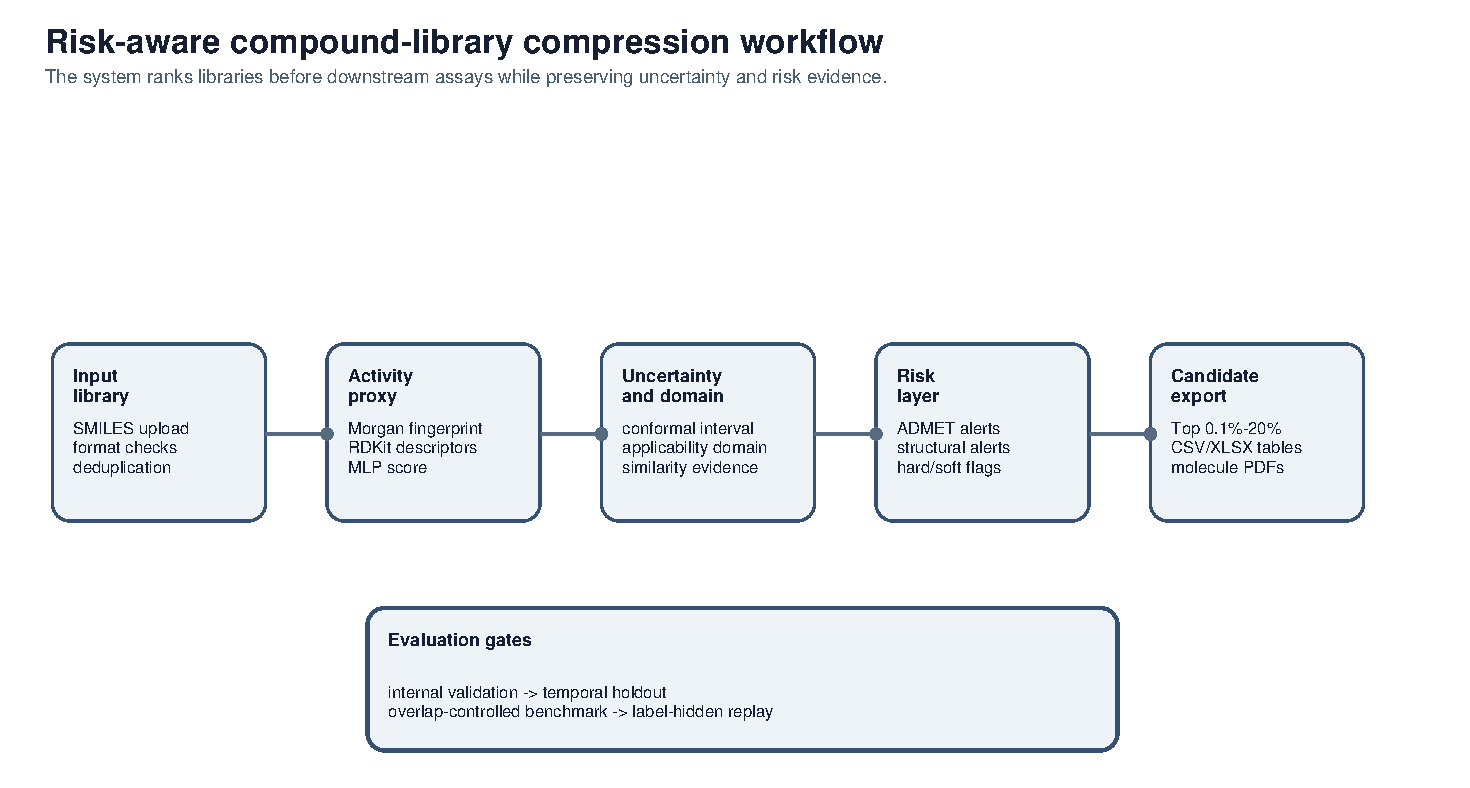
\includegraphics[width=0.95\linewidth]{figures/workflow.pdf}
  \caption{Overview of the risk-aware compound-library compression workflow.}
  \label{fig:workflow}
\end{figure}

\FloatBarrier
\clearpage
\section{Experimental Protocol}
Regression metrics include RMSE, $R^2$ and Spearman correlation. Binary ranking
metrics use the active threshold pChEMBL $\geq 7.0$ and include hit rate,
recall, enrichment factor and NDCG at budgeted cutoffs. For a ranked list with
top-$k$ active rate $h_k$ and full-library active prevalence $p$, enrichment
factor is $EF@k=h_k/p$.

I report three complementary evaluation layers. First, ChEMBL 36 internal
validation and temporal holdout measure how the activity proxy behaves on
frozen split artifacts. Second, overlap-controlled BACE and EGFR subsets test
how the same framework behaves after removing exact standardized-structure or
scaffold matches from training. Third, virtual-batch compression evaluates the
system at batch sizes that resemble external batch submissions rather than single-molecule
benchmarks.

Virtual-batch experiments shuffle each labeled evaluation set into contiguous
batches and evaluate Top-1\%, Top-5\% and Top-10\% ranking quality within each
batch. Five shuffle seeds are used for the main virtual-batch table. Paired
nonparametric bootstrap intervals are computed over frozen prediction rows.
These intervals quantify uncertainty in the fixed prediction artifacts and do
not include model retraining variability.

The strict BACE decision replay uses the official backend API in label-hidden
mode: the system ranks a batch from SMILES only, exports the candidate list,
and restores labels only after the ranking path is complete. This makes the
replay useful for testing the operational path without presenting the library as a
prospective unknown-activity set.

\section{Results}
Figure~\ref{fig:top1} summarizes Top-1\% enrichment across the main evidence
levels. Tables~\ref{tab:model-performance}--\ref{tab:conformal} are generated
directly from machine-readable artifacts in the reproducibility workspace.

\begin{figure}[t]
  \centering
  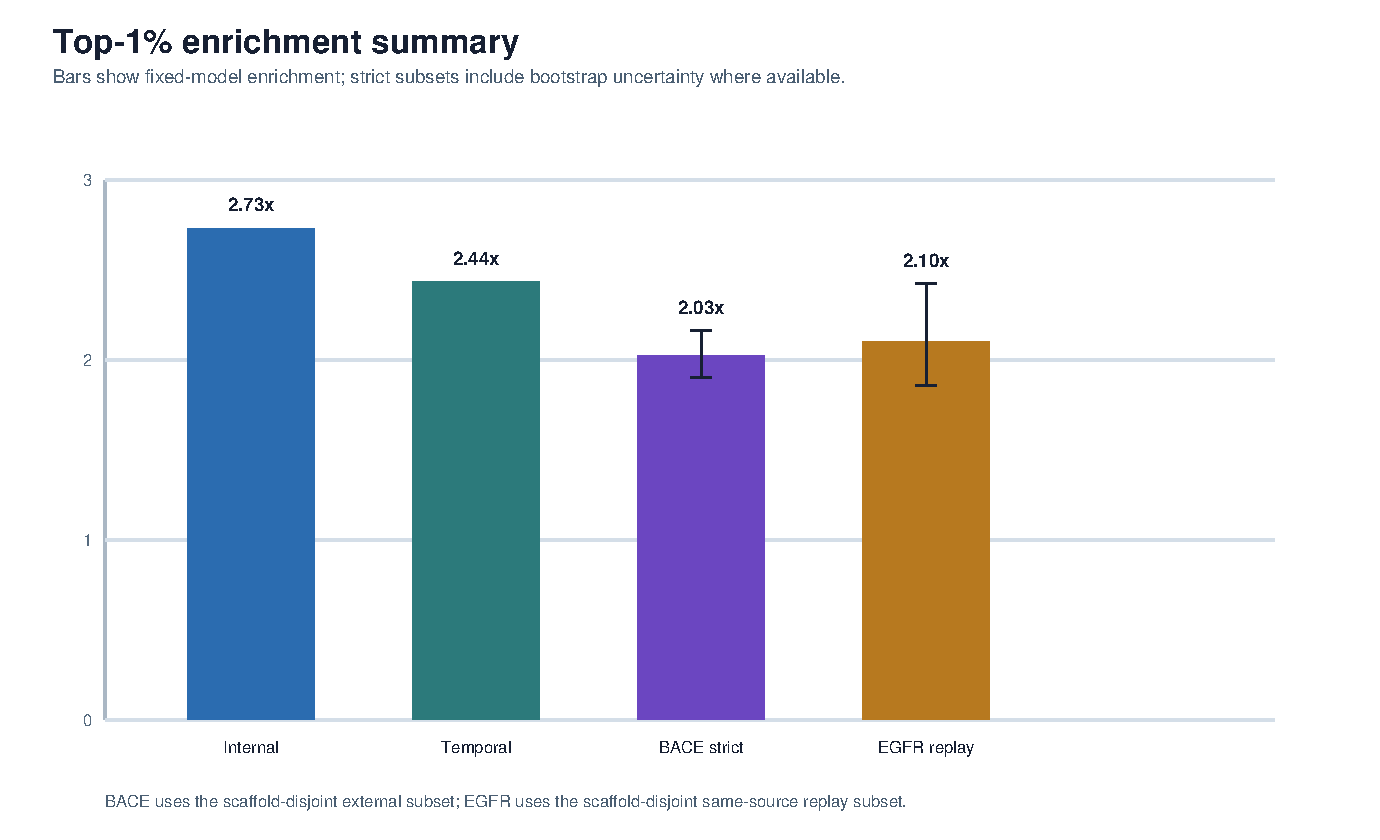
\includegraphics[width=0.95\linewidth]{figures/top1_enrichment.pdf}
  \caption{Top-1\% enrichment on frozen evaluation artifacts: 2.73$\times$
  for ChEMBL 36 internal validation, 2.44$\times$ for ChEMBL 36 temporal
  holdout, 2.03$\times$ for BACE scaffold-disjoint, and 2.10$\times$ for EGFR
  scaffold-disjoint replay. Error bars are shown where bootstrap intervals are
  available for the strict overlap-controlled subsets. BACE uses the
  scaffold-disjoint external subset. EGFR uses the scaffold-disjoint
  same-source replay subset and is not an independent external benchmark.}
  \label{fig:top1}
\end{figure}

On ChEMBL 36, internal validation shows RMSE 0.8466, Spearman 0.7674 and
EF@1\% 2.7331. Temporal holdout performance decreases, as expected under time
shift, but remains useful for ranking with Spearman 0.5171 and EF@1\% 2.4359.
The previous so\_f4 model, random forest and Chemprop checks provide context,
but only the current model and previous so\_f4 future comparison use the full
future artifacts. The sampled random forest and Chemprop rows should therefore
be interpreted as sampled model sanity checks rather than full Future
all-row, same-protocol benchmarks.
\ModelPerformanceTable
\BaselineSanityTable

After removing fold-0 training overlap from BACE, the scaffold-disjoint subset
retains ROC AUC 0.7626, Spearman 0.6047 and EF@1\% 2.0253. This is lower than
the full BACE result, which confirms that overlap control materially changes
the strength of the external claim. The EGFR replay remains strong after
overlap removal, but it is same-source and balanced by construction; it
supports operational sensitivity rather than independent external generalization.
\BaceOverlapTable
\EgfrOverlapTable

The new strict BACE decision replay on a 100-molecule virtual batch shows the
same design trade-off at the system layer. Raw activity sorting gives
Hit@10 of 1.0 and Hit@20 of 0.9, while the risk-aware decision order gives
0.9 and 0.85 on the same batch. That is not a uniform improvement on every
metric; it is evidence that the system changes which compounds are promoted
into the front of the list, making risk and uncertainty visible before the
next experimental round.
\DecisionReplayTable
\FloatBarrier

Table~\ref{tab:strategy-difference} separates two operational questions that
are easy to conflate. The first block shows how much the Top-10 candidate set
changes when selection is driven by activity ranking, scaffold diversity or a
random control on the same BACE scaffold-disjoint artifact. The second block
summarizes the decision buckets observed in the strict 100-molecule BACE
backend replay. These values are a strategy-difference display, not a claim
that any one strategy is uniformly superior under every criterion.
\StrategyDifferenceTable
\FloatBarrier

\subsection{Operational Validation on Simulated Batches}
Operational validation asks whether a budgeted selection rule behaves
differently from simple controls under the same frozen labels. On the BACE
scaffold-disjoint subset, ranking-score selection is compared with random
selection and scaffold-diversity selection at Top 10, Top 50 and Top 100.
The controls are averaged over five seeds. These experiments do not replace
prospective validation, but they provide a practical baseline for evaluating
whether the ranking workflow is doing more than selecting arbitrary or merely
diverse structures.
\OperationalABTable

The same framing can be used for assay-budget accounting. For example, a
10,000-compound library compressed to Top 10\% would produce 1,000 first-round
tests and avoid 9,000 initial tests. Table~\ref{tab:cost-framing} reports this
as an accounting framework and anchors it to the BACE scaffold-disjoint recall
observed in the frozen retrospective artifact. It should not be interpreted as
a project-specific savings claim without external calibration.
\CostFramingTable

The decision matrix in Table~\ref{tab:decision-matrix} summarizes how activity,
uncertainty and domain evidence are combined during review. The matrix is a
reporting abstraction rather than an automatic experimental decision rule.
\DecisionMatrixTable

Across five virtual-library shuffles, the internal, temporal and strict BACE
subsets retain useful early enrichment at a batch size of 1,000. Paired
bootstrap intervals quantify uncertainty in the frozen prediction artifacts,
while the conformal results show that nominal coverage degrades under temporal
shift. Figure~\ref{fig:virtual-batch-trend} visualizes EF@1\% across virtual
batch sizes, supporting the view that early enrichment is not an artifact of a
single batch-size choice. These analyses do not measure model-retraining
variability.
\VirtualBatchTable

\begin{figure}[t]
  \centering
  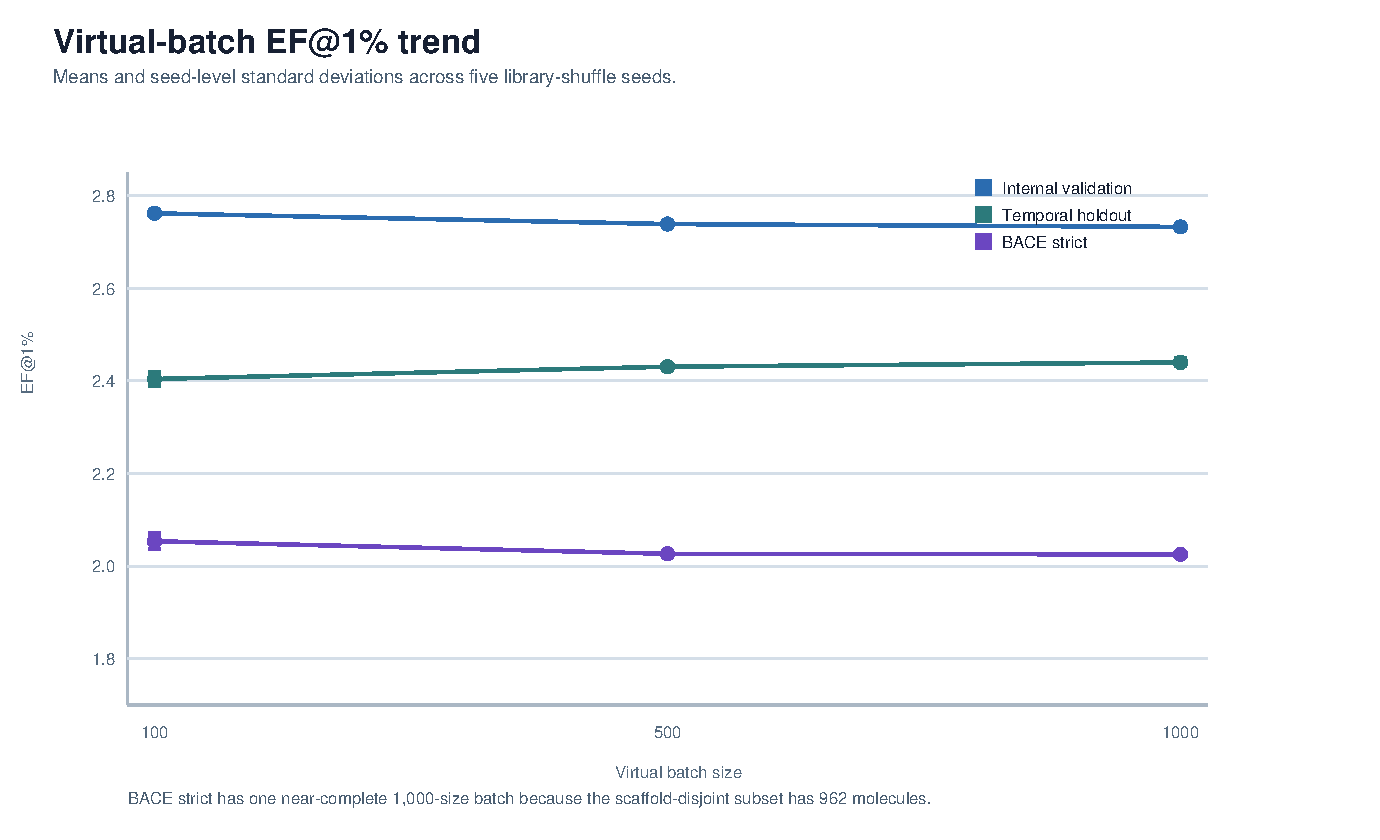
\includegraphics[width=0.95\linewidth]{figures/virtual_batch_trend.pdf}
  \caption{EF@1\% trends across virtual batch sizes. Points show means across
  five library-shuffle seeds; error bars show seed-level standard deviations.
  The BACE scaffold-disjoint row at batch size 1,000 has essentially zero
  variation because the subset contains 962 molecules, so each seed evaluates
  the same single near-complete batch.}
  \label{fig:virtual-batch-trend}
\end{figure}

\BootstrapTable
\ConformalTable
\clearpage

\section{Discussion}
The results support three practical conclusions. First, the current
two-dimensional model is a strong and auditable baseline for early
compound-library compression. Second, Top-$k$ ranking metrics are better
aligned with budget-constrained screening than global regression metrics alone.
Third, leakage auditing can change the interpretation of otherwise impressive
external or replay results, and should be part of the reporting protocol.

For external evaluation, the useful shape of the system is operational: it can
compress a large library into a smaller, reviewable set while preserving the
reasons a collaborator may want to keep, demote or revisit a molecule. That
makes the workflow suitable as an upstream layer for existing pharma, CRO and
supplier screening stacks rather than a replacement for them.

Risk-aware ranking also introduces a deliberate trade-off. A pure activity
ranker may place every high predicted activity molecule at the top, while the
risk-aware layer can demote candidates with uncertainty, applicability-domain
or risk concerns. This is not uniformly superior to activity-only sorting; it
is useful when the decision maker values early visibility into risk and audit
evidence.

For practical use, the framework should be treated as a pre-screening and
review queue rather than as an automatic selection rule. A user with a
100,000-compound library and a first-round experimental budget of 1,000 tests
would start by exporting the Top 1\% candidate set, then inspect ADMET,
structural-alert, uncertainty and applicability-domain fields before choosing
which molecules enter orthogonal testing. The Top 5--10\% lists can be kept as
backup pools for diversity review, procurement constraints, chemistry
feasibility or a second experimental round. When the library is unlabeled, the
appropriate success criterion is not the predicted score itself but the
subsequent enrichment of tested compounds relative to random,
diversity-matched or local-selection baselines. This use pattern keeps the
system aligned with its evidence base: it compresses a large search space,
surfaces risk earlier and preserves an audit trail, while leaving final
experimental decisions to downstream assay results and domain review.

Figure~\ref{fig:virtual-batch-trend} adds a second operational view: early
enrichment remains stable as virtual batch size changes, but the uncertainty
around small external subsets is visibly different from the uncertainty around
large ChEMBL holdouts. This is why I separate frozen-row bootstrap,
shuffle-seed variability and future model-retraining variability instead of
collapsing them into one headline number.

\subsection{Error Analysis and Scope of Validity}
High-ranked inactive molecules are expected in any retrospective screening
artifact, especially under scaffold-disjoint evaluation. Table~\ref{tab:error-cases}
reports three such BACE cases using hashed identifiers. These cases are
interpreted as scope-boundary examples: they show where ranking evidence should
be accompanied by domain, uncertainty and risk review rather than treated as a
standalone activity conclusion.
\ErrorCasesTable

The three cases are informative rather than merely inconvenient. Two have true
pIC50 values just below the active threshold, so the binary inactive label
partly reflects thresholding near a continuous activity boundary. The third is
a stronger miss with a singleton scaffold in the strict subset, which is the
type of case where a target-free 2D prior has limited mechanistic context. The
case with a scaffold frequency of 41 also shows the opposite failure mode:
even when a scaffold is represented inside the strict BACE subset, local
analogs do not guarantee that every member has the same activity. These
examples motivate the risk-aware review layer. The ranking score proposes a
shortlist; it should not be treated as a mechanistic explanation or a final
experimental decision.

The intended interpretation is therefore not that every high-ranked molecule is
active, but that the workflow can enrich early positions while still exposing
the uncertainty and audit information needed to decide whether a molecule
should be advanced, reviewed or deferred.

\section{Limitations}
This paper reports a strong baseline framework rather than a novel molecular
representation. Only one full training fold is currently reported, and the
bootstrap intervals do not include retraining variability. Multi-fold stability
assessment is prepared in the reproducibility workflow, but no partial
multi-fold estimate is reported because incomplete folds would give a false
sense of precision. Public retrospective data cannot establish
project-specific hit-rate improvement or cost reduction. The EGFR replay is
same-source and balanced, and must not be described as a prospective
unknown-activity library. ADMET endpoints vary in temporal generalization;
weak endpoints such as CYP induction should be treated only as low-confidence
review prompts. Prospective or externally blinded experiments are still
required for stronger deployment claims.

\section{Data and Code Availability}
The primary activity records are derived from ChEMBL 36, and BACE is
distributed through MoleculeNet. The manuscript tables and figures are
generated from versioned machine-readable artifacts in the accompanying
reproducibility workspace. The public reproducibility repository is available
at \url{https://github.com/ShengyaoLiang/risk-aware-compound-library-compression}.
Archived releases are indexed under the Zenodo latest-record DOI
\url{https://doi.org/10.5281/zenodo.20833014}.
The non-sensitive source package includes evaluation scripts, dataset
manifests, overlap-controlled public subset files, generated tables and result
artifacts. Runtime account data, external batch submissions, hidden labels,
credentials and business correspondence are excluded from the submission
package. Complete ChEMBL-derived training assets and full train/validation ID
lists are not part of the public package because of size, provenance and
internal-asset boundaries; this is an intentional release boundary rather than
a hidden performance claim. The released artifacts are intended to reproduce
the manuscript tables from frozen non-sensitive summaries and public subset
files.

\section{Conclusion}
Risk-aware compound-library compression offers an auditable interface between
large molecular collections and limited experimental budgets. The present
evidence supports ranking enrichment on internal validation, temporal holdout,
an overlap-controlled external-source BACE subset and a same-source
label-hidden EGFR operational replay. The strongest next validation step is an
externally blinded historical replay or a small prospective A/B experiment
where Top-$k$ candidates are compared against random, diversity-matched, or
existing project-selection baselines. I therefore recommend that interested
groups first run a blinded internal-library replay with the released
non-sensitive artifacts and then, if enrichment is observed, design a
prospective A/B pilot to measure project-specific hit-rate, time and assay
budget effects. In practice, this makes the framework a reproducible
pre-screening layer: it reduces the first-round search space, surfaces risk
earlier, and keeps the audit trail intact.

\appendix
\section{Supplementary Material: System Interface Specification}
The reference implementation accepts plain SMILES as the minimal molecular
input. Optional metadata can include a batch name, row identifier and
non-sensitive user-side labels for local traceability, but target names,
project codes and biological context are not required for the target-free
ranking pass. Standard output artifacts include:
\begin{itemize}
  \item Top-$k$ CSV/XLSX files for budgeted library review;
  \item molecule-level PDF reports for selected candidates;
  \item audit fields for ranking score, uncertainty, applicability-domain
        evidence, structural alerts and risk categories; and
  \item provenance records linking exports to batch identifiers and frozen
        software/model artifacts.
\end{itemize}

Typical integration points include workflow systems such as KNIME, Pipeline
Pilot, Spotfire-style dashboards, ELN/LIMS imports and internal data lakes. The
export contract is intentionally tabular so that downstream groups can consume
candidate lists without adopting a specific user interface. Account-level
isolation was used in the operational replay environment; an external
deployment should additionally define transport security, retention policy,
access control, logging and incident-response procedures.

\section{External Validation Protocols}
Two validation protocols are recommended for external calibration. In a
blinded retrospective replay, an external group provides SMILES while holding
back labels. The system ranks and exports Top-$k$ candidates, after which the
external group reveals labels for EF, hit-rate, recall and NDCG estimation.
This protocol is low-cost and directly tests whether the ranking layer adds
value relative to random or diversity-based controls in that data context.

In a prospective A/B pilot, candidate sets are selected by the ranking
workflow, by random or diversity-matched controls, and by an existing local
selection process if one is available. Experimental readouts are then compared
after testing. This is the appropriate protocol for project-specific hit-rate
or cost claims; such claims are not made from the retrospective public
benchmarks in this paper.

\section*{Author Contributions}
Shengyao Liang conceived and designed the study, prepared and evaluated the
datasets and models, implemented the reproducibility workflow, analyzed the
results, and wrote the manuscript.

\section*{Funding}
This work received no external funding.

\section*{Competing Interests}
The author declares no competing interests.

\bibliography{references}
\end{document}


